\chapter{Evaluation}\label{ch:evaluation}

We now evaluate and analyse our designs using a series of different benchmarks and running
the system under different configurations. We run all benchmarks on the
Freescale i.MX 8M Mini quad applications processor with 2GB RAM, running at 1.2 GHz
with a 1Gbps NIC. The configurations for each system tested are specified by each benchmark,
and the system comprises of the following PDs:
\begin{enumerate}
    \item Ethernet Driver
    \item (only as specified) Client Side Ethernet Driver
    \item Rx Mux
    \item Tx Mux: implementation specified in each benchmark
    \item ARP Component
    \item Timer Driver
    \item 1 Rx Copy Component per Client application
    \item 1 or more Client applications as specified in each benchmark. 
        The clients use lwIP \cite{Dunkels_01} as an IP stack library for network packet processing. 
    \item (only as specified) Tx Copy Component
\end{enumerate}

For all echo applications, we use ipbench as a distributed load generator 
to send 1472 byte-sized UDP packets to test the seL4 based system. ipbench runs on a 4-node x86 cluster, 
connected to the same switch as our test system,
and counts the number of successful replies from the target system to measure the achieved throughput and latencies.
All benchmarks use a sample size of 200,000 packets unless otherwise specified. 

For all asymmetric client applications, we implement our own custom benchmarking applications to run on an Intel Xeon W-1250
running at 3.3 Ghz, with 64GB RAM and equipped with a 10Gbps NIC. For our transmit-dominant client, our benchmarking
application receives packets using \emph{recv()} and records start and stop time to determine the total transmitted
throughput. For our receive-dominant client, our benchmarking application transmits packets using \emph{send()} and
we count the number of successfully received packets by the client itself to determine the total received throughput.

We also compare some echo server configurations against a Linux system (version 6.1.1) on the same hardware. 
We use a simple user level application which reads and then writes all packets immediately back using the socket API. 
In order to determine the CPU utilisation of both systems, we run an idle thread on each core
at low priority to count the number of idle cycles of that core. 

\section{Asymmetric Client Applications}

Our asymmetric client applications demand significantly more throughput in one direction compared to the 
other. We implement each of the client applications as per \autoref{s:client_apps}.
We measure the total received throughput by a receive-dominant application (Rx Mostly), the
transmitted throughput by a transmit-dominant application (Tx Mostly) and the transmitted throughput
of a client-initiated transmit application (Tx Initiated) and compare these tests against the achieved
throughput of the echo server. 

\vspace{0.5cm}
\begin{figure}[h]
    \centering
    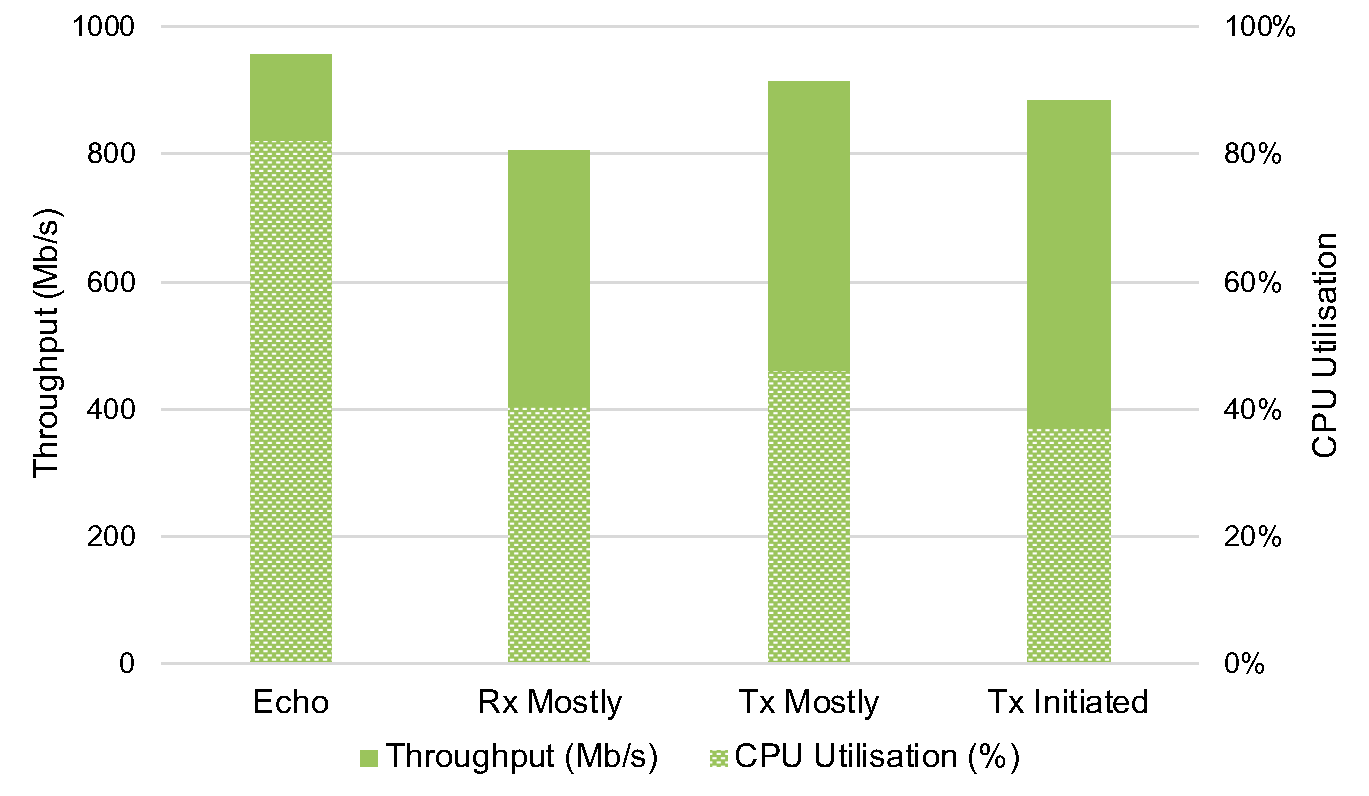
\includegraphics[width=0.6\textwidth]{asym.pdf}
    \caption{Networking Performance of Different Client Applications}
    \label{f:asym}
\end{figure}

\autoref{f:asym} shows the measured throughput as well as the CPU utilisation of each test application. 
Compared with our echo benchmarks, our asymmetric applications both utilise 50\% less CPU for 80+\% of the
throughput. While we would be able to achieve higher throughput in these examples by receiving/sending
more than 10,000 packets for every packet in the other direction, this would defeat the purpose of these examples.
From both of these results, we can conclude our system is able to cope well with asymmetric UDP traffic. 
In our client initiated benchmark, we are able to achieve near wire speed with less than 40\% CPU. This is inline
with our expectations compared to our echo benchmarks, given this system has half the workload with no incoming
packets. Although these tests are fairly simple, they provide a good sanity check to confirm our system can 
keep up with different workloads and present a good starting point for developing more complex workloads in the future.

\section{Multi-client systems}

Our design has a large number of different parameters to experiment with, including multiplexer
policies, queue sizes and the scheduling parameters of client applications running on the system. 
We select a small variety of example systems to evaluate our different policy designs. We evaluate
these systems with two separate ipbench instances running on different clusters sending UDP packets
at the same time to their respective clients.

We start first with evaluating single core configurations running two echo server applications. 
Each system comprises of an Ethernet driver, Rx Mux, Tx Mux, 2 copy components (1 for client A, 1 for client B) 
and two simple echo servers; client A and client B. As these systems run on single core, a round robin or priority-based
policy in the Tx Mux would not make sense as the multiplexer runs at higher priority than both the clients and thus
will be invoked as soon as it is signalled by either client. We instead first evaluate a simple Tx Mux that only 
responds to the client that signalled it, and enforce policy through our system design. We also evaluate our
bandwidth limited multiplexer on its ability to efficiently enforce different bandwidth limits for different clients.

We first evaluate a system where both clients run at equal priority, with their respective copy components at 
equal, higher priority than their client, and both clients have a queue size of 512 for all interfacing queues.

\noindent\begin{figure}[H]
    \centering
	\begin{multicols}{2}
		\begin{subfigure}[b]{0.45\textwidth}
        \centering
        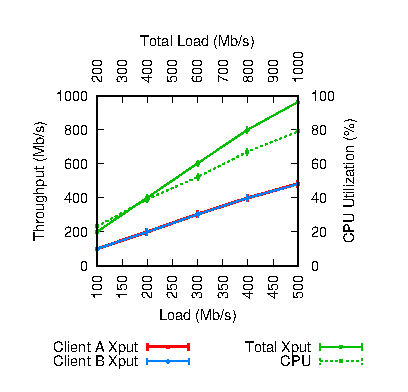
\includegraphics[width=1.2\textwidth]{AB.eps}
        \caption{Networking Performance of Two Echo Servers at Equal Priorities}
        \label{f:AB}
    \end{subfigure}\qquad
    \begin{subfigure}[b]{0.45\textwidth}
        \centering
        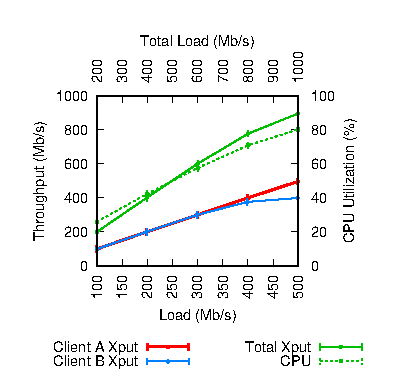
\includegraphics[width=1.2\textwidth]{AB_RxU16.eps}
        \caption{Networking Performance of Two Echo Servers at Equal Priorities, with limited RxU Queue of Client B}
        \label{f:AB_Rx16}
    \end{subfigure}
\end{multicols}
\end{figure}

\autoref{f:AB} shows the achieved throughput for client A and B and the CPU utilisation of the entire system. 
Both clients achieve the same throughput, and their combined total reaches wire speed.\\

We now limit the RxU queue between the Rx Mux and the copy component of client B to just 16 to measure 
the impact this will have on client B's throughput. \autoref{f:AB_Rx16} shows the resulting network performance.
Client A still achieves the requested throughput but client B is limited to 400Mbps. This is because the RxU queue
to client B will become full much sooner, causing the Rx Mux to discard subsequent packets for client B and thus
limiting the total throughput available to client B. 

We now incorporate different priorities to our system and measure the impact this has on each clients
achieved performance. We reduce both client B and its copy component to lower priority than client A. 
Thus the priorities are ordered as follows:\\ 

\centerline{Driver \(>\) Tx Mux  \(>\) Rx Mux \(>\) ARP \(=\) Copier of client A \(>\) client A \(>\) Copier of client B \(>\) client B.}

We set all queue sizes to be equal. 

\noindent\begin{figure}[H]
    \centering
	\begin{multicols}{2}
		\begin{subfigure}[b]{0.45\textwidth}
        \centering
        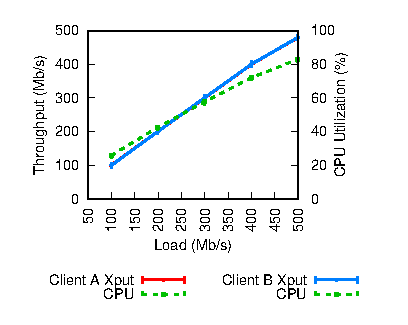
\includegraphics[width=1.2\textwidth]{AgtB_RxU32.eps}
        \caption{Throughput Achieved by each Client}
        \label{f:AgtB_RxU32_xput}
    \end{subfigure}\qquad
    \begin{subfigure}[b]{0.45\textwidth}
        \vspace{39pt}
        \centering
        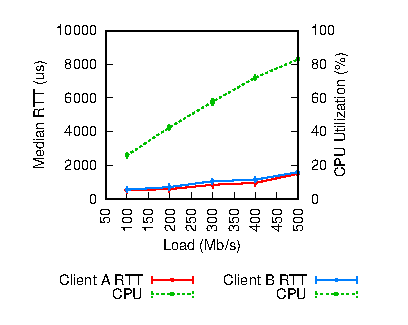
\includegraphics[width=1.2\textwidth]{AgtB_RxU32_latency.eps}
        \caption{Median Latencies for each Client}
        \label{f:AgtB_RxU32_latency}
    \end{subfigure}
\end{multicols}
\caption{Networking Performance of Two Echo Servers at Different Priorities}
\label{f:AgtB_RxU32}
\end{figure}

We see in \autoref{f:AgtB_RxU32_xput} the throughput of the lower priority client remains unaffected as there isn't enough
contention on the CPU to limit this clients CPU bandwidth and both clients achieve their requested load.
However, the latencies are affected by this. \autoref{f:AgtB_RxU32_latency} shows the median round trip time (RTT)
for each client. Client A achieves lower latencies than client B as it is running
at higher priority and thus is scheduled to run first.

If there was more contention for the CPU, then we would expect the priority assignment of each client to have an effect
on their achieved throughput. We now add unnecessary overhead to each packets round trip to simulate an environment where
this is the case. We have each client copy each packet and calculate a checksum 10 times as per \autoref{s:compute_heavy}. 

\noindent\begin{figure}[H]
    \centering
	\begin{multicols}{2}
		\begin{subfigure}[b]{0.45\textwidth}
        \centering
        \includegraphics[width=1.2\textwidth]{AgtB_overload.eps}
        \caption{Equal Queue Sizes}
        \label{f:AgtB_overload}
    \end{subfigure}\qquad
    \begin{subfigure}[b]{0.45\textwidth}
        \centering
        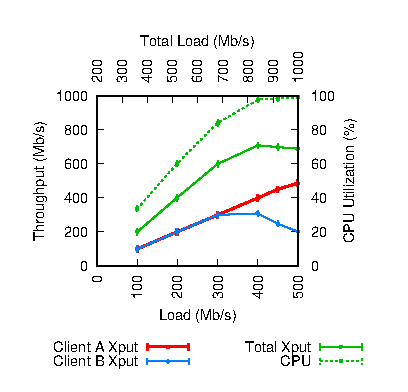
\includegraphics[width=1.2\textwidth]{AgtB_RxU32_overload.eps}
        \caption{Limit RxU Queue of Client B to 32}
        \label{f:AgtB_RxU32_overload}
    \end{subfigure}
\end{multicols}
\caption{Networking Performance of Two Overloaded Echo Servers at Different Priorities}
\label{f:AgtB_od}
\end{figure}

\autoref{f:AgtB_overload} shows the achieved throughput for both clients. Neither client achieves its requested load, with client A,
the higher priority client, maxing out at 400Mbps and client B seeing a performance collapse to 300Mbps. By the total achieved throughput
and CPU load, it is clear the system is overloaded at this point. However, it is clear that client B as the low priority client is 
starving client A by monopolising shared Rx buffers, as client A is not able to achieve its requested load. We now limit client B's RxU queue
to 32 to prevent this and ensure there are adequate Rx buffers available to higher priority clients as per \autoref{s:rx_policy}. 
\autoref{f:AgtB_RxU32_overload} shows the resulting performance. The total throughput achieved is not affected by this change, and the
system still becomes overloaded at 400Mbps. However, client A is now able to achieve its requested load as client B's available
Rx throughput is limited. \\

The results all indicate that limiting a clients queues will limit its available throughput. We can use this property to implement 
a bandwidth-limited policy in the system. We now limit the RxU queue between the Mux and Copier of client B to just 16, and also
limit the TxU queue between the Mux and client B to 16. Client B and its Copier still run at lower priority than client A, and both
clients are just simple echo servers (with no additional overload).

\begin{figure}[h]
    \centering
    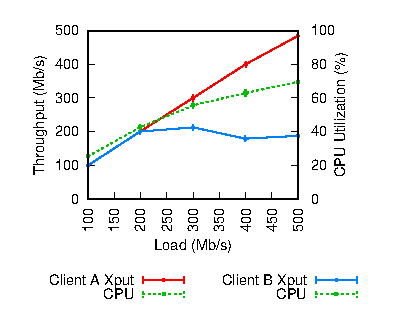
\includegraphics[width=8cm]{AgtB_RxTxU16.eps}
    \caption{Networking Performance of Two Echo Servers with Limited Queues to Client B}
    \label{f:AgtB_RxTxU16}
\end{figure}

\autoref{f:AgtB_RxTxU16} shows the resulting performance. Client A still achieves its requested load, but client B is limited
to just 200Mbps. The total CPU load is also reduced compared to the system without any queue limits, indicating less load on 
the limited client.

\subsection{Bandwidth-limited Tx Multiplexer}

We can also limit clients available bandwidth using policy in the Tx Mux. We evaluate \autoref{s:bandwidth} with two echo servers,
running at equal priority and with equal queue sizes, and limit client B to just 100Mbps in the Tx Mux. Client A is not limited.

\begin{figure}[H]
    \centering
    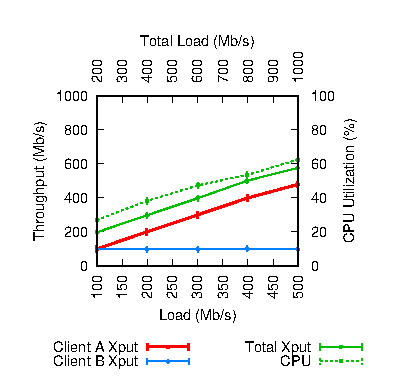
\includegraphics[width=8cm]{Tx_Limited.eps}
    \caption{Networking Performance of Two Echo Servers with Bandwidth-Limited Multiplexer}
    \label{f:Tx_Limited}
\end{figure}

\autoref{f:Tx_Limited} shows the achieved throughput for both clients and the total CPU load of the system. As expected, 
client A which does not have a bandwidth limit, achieves its requested load and client B is limited to just 100Mbps. Furthermore, 
the total CPU load for the total achieved throughput (600Mbps) is only 62\%. Compared to the CPU load of the same 
achieved throughput without any bandwidth limiting (see \autoref{f:AB}) of 52\%, this is less than a 20\% increase. While we
expect there to be some overhead as the multiplexer must communicate regularly with a timer driver, thus incurring additional
context switches, some of this overhead can be reduced with an optimised implementation 
as outlined in \autoref{s:bandwidth}. This is left for future work.

In order to properly evaluate our round robin and priority-based multiplexer designs, we must first evaluate how our
design scales to multi-core. From there, we can design systems where the clients run on separate cores and will be scheduled irrespective
of one another, thus requiring further policy in the multiplexer.

\section{Multi-core}

Scaling to multi-core will incur overhead from two separate causes. Firstly, seL4 configured with symmetric multi-processing (SMP) increases
the cost of every kernel invocation. This is not only due to the cost of acquiring the kernel lock, but also because the SMP kernel is
less optimised and some fast paths do not apply. Secondly, inter-core communication costs significantly more than intra-core due to the addition of 
inter-processor interrupts (IPI) for inter-core signalling and cache-line bouncing from any shared data. While detailed analysis of these overheads is left for future work, in order to properly
analyse how our system performs on multi-core configurations, we first establish a baseline of these costs. We first evaluate two separate configurations
using the SMP kernel: pinning every component to a single core and splitting the load across two cores (out of an available 4). 
We compare these to our baseline without the SMP kernel. Each system is comprised of 5 PDs: an Ethernet driver, RX Mux, 
TX Mux, Copy Component, Client running a simple echo server. Our two core system pins the driver and Tx Mux to one core, and 
the Rx Mux, Copier and Client pinned to the other. We also compare these systems against a typical Linux set up, whereby
the user-space echo server application is pinned to one core, and we allow the Linux scheduler to schedule the remaining 3 cores.\\ 

\begin{figure}[H]
    \centering
    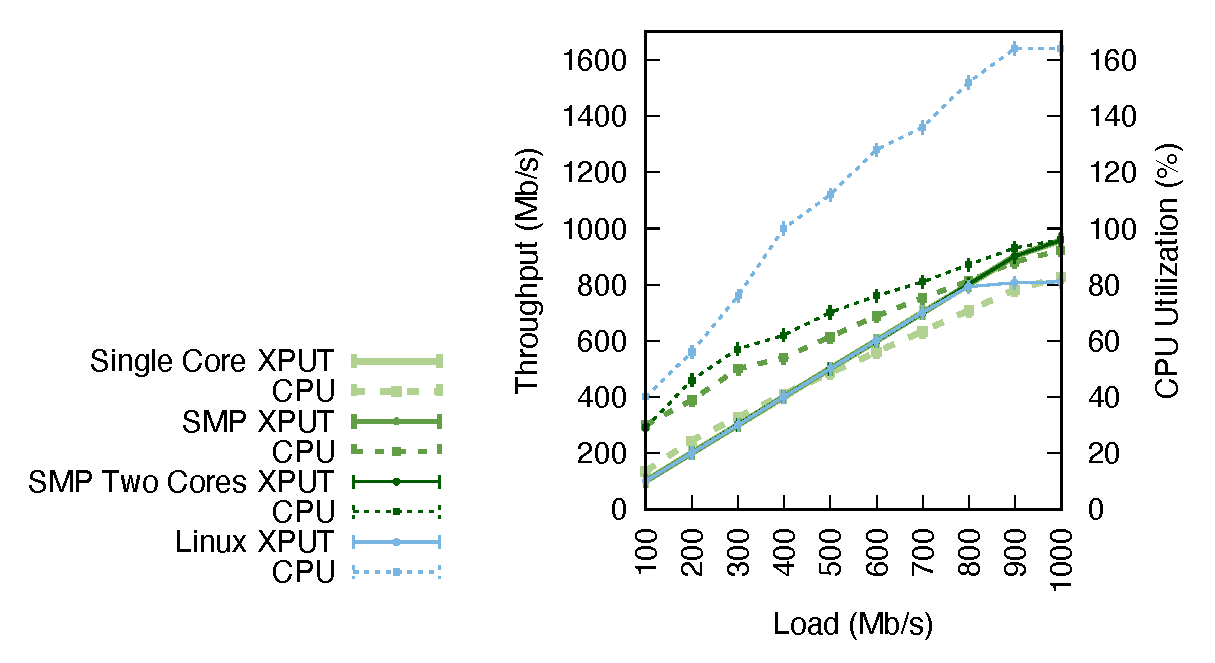
\includegraphics[width=0.9\textwidth]{multicore.pdf}
    \caption{Networking Performance Comparison of Multi-core Systems}
    \label{f:multicore}
\end{figure}

\autoref{f:multicore} shows the achieved throughput against the CPU utilisation for our 3 different seL4-based systems and Linux. 
As expected, each of our 3 seL4-based systems achieve wire speed (the paler, solid green lines are directly behind the dark green line)
whereas the Linux system maxes out at just 800Mbps. All seL4 systems also outperform the Linux system, which utilises more than
1.6 cores for 800Mbps. Further investigation into the Linux system reveals the core running the echo server is maxed out at 
this point, and hence why the system can't achieve higher throughput. \\
However, the total CPU utilisation of each of our seL4 systems differs substantially. 
The difference between the single core CPU load (dotted, pale green line) and the single core SMP CPU load (dotted mid-green line) 
outlines the overhead of using the SMP kernel. To achieve wire speed, the normal kernel configuration utilises 82\% of the CPU, whereas
the SMP kernel configuration utilises 92\% of the CPU; about 12\% overhead. While this is substantially higher than expected given
there is no inter-core communication for either of these configurations, detailed
exploration of these overheads is left for future work. 
Comparing the single core SMP CPU load against the two core SMP CPU load (dotted dark green line) outlines the overheads introduced by
inter-core communication between our 5 PDs; just over 4\% at wire speed. Note that not all system calls will introduce IPIs in
this configuration, as, for example, the Copy component only communicates intra-core with the Rx Mux and Client. \\

Ultimately, distributing PDs across different cores will incur different overheads. We explore these overheads with another benchmark
comparing 4 separate configurations. Each different configuration isolates one PD on one core, and runs all other PDs on another core. 
We test these configurations with the same echo server benchmark with the same 5 PDs as our previous multi-core benchmark.

\begin{figure}[H]
    \centering
    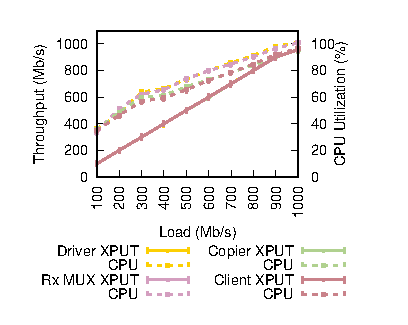
\includegraphics[width=10cm]{multicore_distr.eps}
    \caption{CPU Utilisation with Select Components Isolated on a Separate Core}
    \label{f:multicore_distr}
\end{figure}

\autoref{f:multicore_distr} shows the results when isolating the driver, Rx Mux, Copier and Client. The yellow lines show the throughput
and CPU utilisation when the driver is pinned to a separate core. Likewise, the purple for the Rx Mux, the green for the Copier and pink for
the Client. As expected, each different configuration achieves wire speed but the CPU utilisation of each system differs. Notably, 
the configuration where the driver is isolated incurs the most overhead, followed closely by the configuration isolating the Rx Mux. This is 
expected due to the higher number of system calls per packet each of these PDs makes and thus these systems will incur more overheads from
intra-core signalling and kernel lock contention. Overall, the difference in CPU load of each of these systems is only 4\%, indicating that
components can be arbitrarily distributed across cores. Ultimately, the optimal allocation for a system is use case dependent.\\
Now we have a baseline evaluation for multi-core systems, we can design simple systems with which to evaluate our other transmit multiplexer
designs. 

\subsection{Round Robin Tx Multiplexer}

A round robin policy in our Tx Multiplexer only makes sense when clients are running on separate cores. This is because the Tx Mux runs at higher
priority than the clients, and will be invoked as soon as a client has signalled it. If both clients are on the same core, then the Tx Mux will
be invoked after one client has finished enqueuing packets for transmit, but before the other client has been scheduled. We evaluate our round robin
Tx Mux on a 2 client multi-core configuration, where each client is pinned to a separate core shared with its respective copy component, and another
core hosts the Driver, Rx Mux, ARP Component and Tx Mux. 

\noindent\begin{figure}[H]
    \centering
	\begin{multicols}{2}
		\begin{subfigure}[b]{0.45\textwidth}
        \centering
        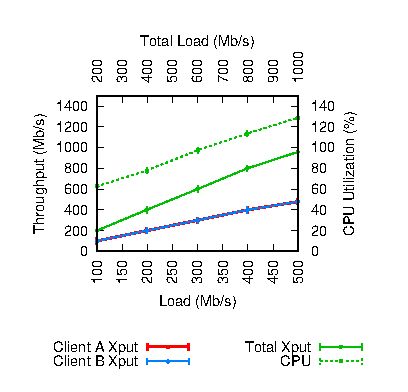
\includegraphics[width=1.2\textwidth]{Tx_Round_Robin.eps}
        \caption{Throughput Achieved and CPU Load of Two Echo Servers}
        \label{f:round_robin_mux}
    \end{subfigure}\qquad
    \begin{subfigure}[b]{0.45\textwidth}
        \vspace{52pt}
        \centering
        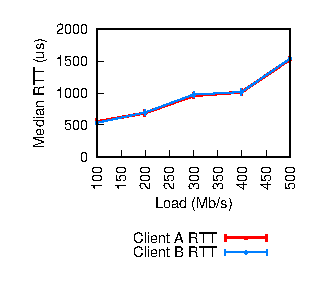
\includegraphics[width=\textwidth]{Tx_Round_Robin_latency.eps}
        \vspace{0.5pt}
        \caption{Median Latencies of Two Echo Servers}
        \label{f:round_robin_mux_latency}
    \end{subfigure}
\end{multicols}
\caption{Networking Performance of Two Echo Servers with a Round Robin Multiplexer}
\end{figure}

The total achieved throughput as well as that of each client is shown in \autoref{f:round_robin_mux}. As expected, both clients achieve their 
requested throughput, with their sum equalling wire speed. Importantly, both clients experience the same networking latencies as shown
in \autoref{f:round_robin_mux_latency} by their respective median round trip times. This demonstrates our round robin Tx Mux enforces
fairness between two clients effectively.\\

The system incurs significant overhead than when compared to our equal priority, single core example in \autoref{f:AB}. To
achieve a total of 200Mbps (100Mbps per client), our multi-core system utilises 63\% of the CPU (split across 3 cores) compared with 
only 23.5\% CPU utilisation of our single core example. To better understand these overheads, we run our equal priority, 
single core example again (see \autoref{f:AB}) but with the SMP kernel instead. We find that to achieve
a total throughput of 200Mbps, the system utilises 51\% of the CPU, and the system maxes out at just over 700Mbps. 
From this we can conclude that most of the overheads in these systems stem 
from just using the SMP kernel, and an additional 22\% accounts for the costly intra-core communication across 3 cores as 
well as any overheads of the multiplexer itself.

\subsection{Priority-based Tx Multiplexer}

We also evaluate our priority-based Tx Mux using the same system design, where we will instead expect a higher priority client to achieve smaller
latencies. We set up our priority-based Tx Mux implementation to prioritise client A, followed by client B and finally ARP at lowest priority.
As both clients run on separate cores, their scheduling parameters with respect to one another has no impact and so we allocate them the same
scheduling priority as one another. Likewise with their copy components, which are higher priority than the client. 

\noindent\begin{figure}[h]
    \centering
	\begin{multicols}{2}
		\begin{subfigure}[b]{0.45\textwidth}
        \centering
        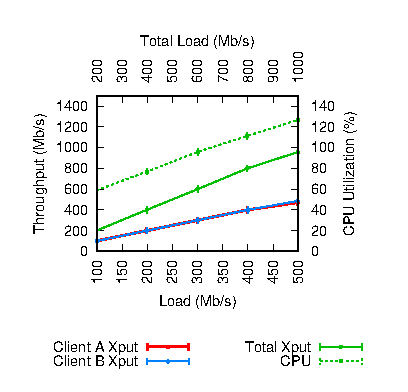
\includegraphics[width=1.2\textwidth]{Tx_Priority.eps}
        \caption{Throughput Achieved and CPU Load of Two Echo Servers}
        \label{f:priority_mux}
    \end{subfigure}\qquad
    \begin{subfigure}[b]{0.45\textwidth}
        \vspace{52pt}
        \centering
        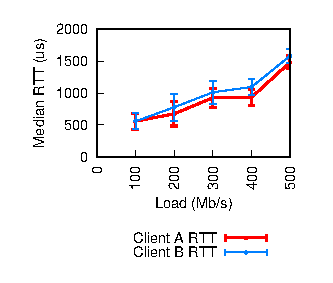
\includegraphics[width=\textwidth]{Tx_Priority_latency.eps}
        \vspace{0.5pt}
        \caption{Median Latencies of Two Echo Servers}
        \label{f:priority_latency}
    \end{subfigure}
\end{multicols}
\caption{Networking Performance of Two Echo Servers with a Priority-based Multiplexer}
\end{figure}

Both clients achieve their requested throughput as shown in \autoref{f:priority_mux} and as expected, \autoref{f:priority_latency} shows
that client A has lower latencies over client B. Notably, client A's latencies are also lower on this system, with a median RTT
of 1480us at wire speed, when compared to our system with a round robin policy, where client A has a median RTT of 1524us at the same
throughput. This demonstrates our policy implemented in the Tx Mux works effectively to prioritise
client A over client B.\\
Furthermore, both our round robin multiplexer and our priority-based multiplexer introduce similar overheads as indicated by their 
respective CPU utilisation measurements. \\

\newpage

\subsection{Two-threaded Driver}
For some multi-core systems, the driver could be a performance bottleneck if the core it is running on is saturated. We can offload
some of the drivers work to another core with our two-threaded driver design. In doing so, we will introduce additional overheads
stemming from an additional context switch per packet, as well as communication between the two driver components required at
high loads. We first measure these overheads by comparing our single core system with a simple echo server client against the 
same system with our two threaded driver design. We compare the overall throughput and CPU utilisation of both systems. As 
our two-threaded driver design is only applicable in multi-core systems, we configure both systems with SMP enabled but 
initially confine them to a single core.

\begin{figure}[h]
    \centering
    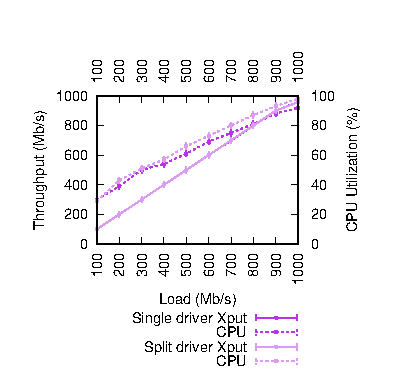
\includegraphics[width=8cm]{2driver_comp.eps}
    \caption{Performance Comparison of Two Threaded Driver on Multi-core}
    \label{f:2driver_comp}
\end{figure}

\autoref{f:2driver_comp} shows the results. Both systems achieve the total requested throughput. The CPU utilisation of our 
two-threaded driver (pink dotted line) shows that at low throughputs, the overhead is minimal. However, at high loads, we
see a 6\% increase in CPU load.\\

We now design a system where the two-threaded driver design may be applicable. The driver will only be a bottleneck in a
multi-core system when the core it is running on is saturated, and there are no other available cores with sufficient bandwidth
to run the driver on. To replicate such a scenario, we configure our system with 4 compute-heavy client applications. We set up
4 echo servers to copy each packet 100 times and calculate a checksum 100 times. We configure each client to run on its own
core, along with its copy component, and use our round robin transmit multiplexer to ensure fairness across the clients. 
As our hardware platform only has 4 cores, the driver must share a core with at least one client and 
its copy component. The core assignment is as follows:
\begin{itemize}
    \item[\textbf{Core 0:}] Driver, Copier of client A, client A
    \item[\textbf{Core 1:}] Rx Mux, Copier of client B, client B
    \item[\textbf{Core 2:}] Copier of client C, client C
    \item[\textbf{Core 3:}] Tx Mux, Copier of client D, client D
\end{itemize}

We test this system with 4 separate ipbench instances, each sending UDP packets to a client and counting received packets
to determine throughput achieved by this client. We request up to 250Mbps for each client for a combined total of 1Gbps on the system.

\begin{figure}[h]
    \centering
    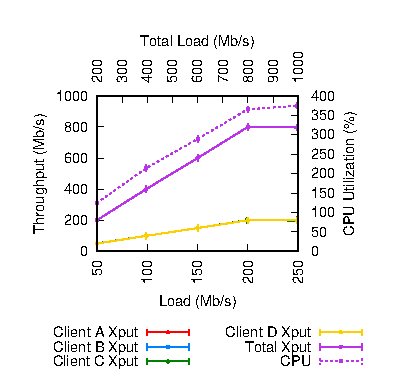
\includegraphics[width=8cm]{multicore_overload.eps}
    \caption{Networking Performance with 4 Clients on Multi-core}
    \label{f:multicore_overload}
\end{figure}

\autoref{f:multicore_overload} shows the achieved throughput for each client, as well as the total throughput achieved 
by the system and the total CPU load. Each client is able to achieve 200Mbps but no more. We now configure this system 
with our two-threaded driver, and offload some of the drivers work to core 2 to test whether clients are able to 
achieve higher load. The core assignment is as follows:

\begin{itemize}
    \item[\textbf{Core 0:}] IRQ-side Driver, Copier of client A, client A
    \item[\textbf{Core 1:}] Rx Mux, Copier of client B, client B
    \item[\textbf{Core 2:}] Client-side Driver, Copier of client C, client C
    \item[\textbf{Core 3:}] Tx Mux, Copier of client D, client D
\end{itemize}

\begin{figure}[h]
    \centering
    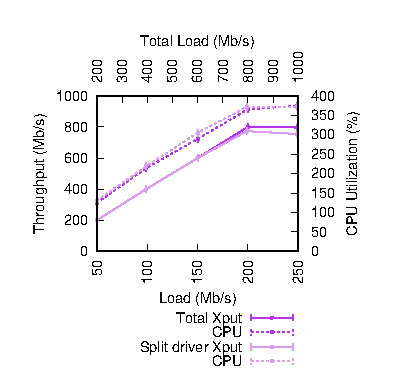
\includegraphics[width=8cm]{2driver_comp_overload.eps}
    \caption{Performance Comparison of Two Threaded Driver with 4 Clients on Multi-core}
    \label{f:2driver_comp_overload}
\end{figure}

\autoref{f:2driver_comp_overload} shows the performance comparison of both systems total throughput achieved and CPU load. 
The system with the two-threaded driver actually achieves slightly lower throughput than the system with the single driver
at the same CPU load. We now take a closer look at the CPU utilisation of each core.

\noindent\begin{figure}[H]
    \centering
	\begin{multicols}{2}
	\begin{subfigure}[b]{0.45\textwidth}
        \centering
        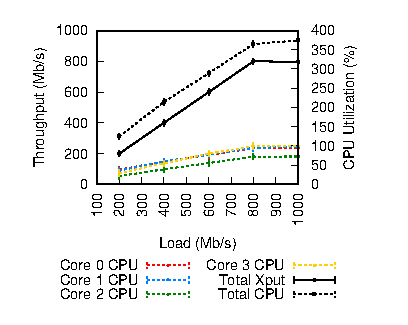
\includegraphics[width=1.2\textwidth]{core_analysis_multicore_overload.eps}
        \caption{Single driver system}
        \label{f:core_analysis_mutlicore_overload}
    \end{subfigure}\qquad
    \begin{subfigure}[b]{0.45\textwidth}
        \centering
        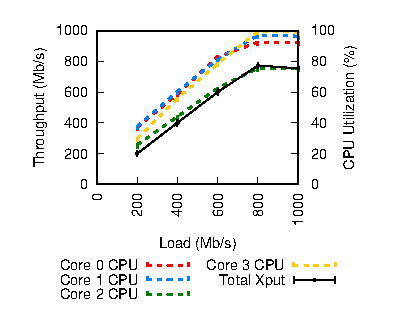
\includegraphics[width=1.2\textwidth]{core_analysis_multicore_overload_2driver.eps}
        \caption{Two-threaded driver system}
        \label{f:core_analysis_mutlicore_overload_2driver}
    \end{subfigure}
\end{multicols}
\caption{Core Utilisation of an overloaded 4 Client System }
\label{f:core_util_multi}
\end{figure}

\autoref{f:core_util_multi} shows each cores utilisation against the requested load for both systems. 
In both systems cores 0, 1 and 3 are all saturated. This tells us that although the driver is a potential
bottleneck, both the Rx and Tx multiplexers are too. In \autoref{f:core_analysis_mutlicore_overload_2driver}
we see core 0 has slightly lower utilisation at wire speed compared with
\autoref{f:core_analysis_mutlicore_overload_2driver}, showing that our two-threaded driver design has successfully
offloaded some of the driver load to another core. However, as our multiplexers are also both bottlenecks in 
this example workload, the two-threaded driver design is not enough to improve performance. We hypothesise that
splitting the multiplexers into two separate components, one component responsible for processing used packets and 
the other for processing free packets, may help reduce load on those cores, but such a design is only applicable
on systems with more available CPUs. We leave this exploration for future work.

\section{Transmit Copy Component}

We now measure the overheads introduced by our additional transmit copy component. We implement a new
component between the Tx Mux and our client application as per \autoref{f:tx_copy}. While the implementation
of this component depends on system design and the threat scenario, we measure the total possible overhead
added if the component is responsible for all possible tasks listed. These are:
\begin{itemize}
    \item Ensuring metadata enqueued to the multiplexer is sane.
    \item Checking outgoing packets are well-formed 
    \item Copying outgoing packets into a separate region not mapped
          into the clients address space.
    \item Interfacing with the multiplexer correctly by incrementing the head/tail pointers as required.
    \item Ignoring any transmit packets from the client that do not abide by the protocols.
\end{itemize}

We measure these overheads on a simple echo server system. We run this new component at higher priority than the client
and the Rx Copy component to ensure invocation as soon as packets are ready to be transmitted and thus keep
latencies low. We use a simple Tx Mux with no explicit policy and the priority assignment of the system is as follows:\\
\centerline{Driver \(>\) Tx Mux  \(>\) Tx Copy \(>\) Rx Mux \(>\) Rx Copy \(>\) Client}

We compare the achieved throughput and CPU utilisation of this system to the same system without this additional component. 

\begin{figure}[h]
    \centering
    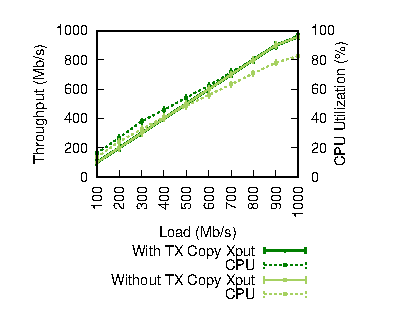
\includegraphics[width=10cm]{tx_copy_overhead.eps}
    \caption{Performance Overhead with Tx Copy Component}
    \label{f:tx_copy_overhead}
\end{figure}

\autoref{f:tx_copy_overhead} shows the resulting performance with and without the Tx Copy component. As expected, both
systems achieve wire speed. At 100Mbps, our system utilises 16\% CPU with our Tx Copy component, compared to 13.5\% CPU 
without the additional component. This is about an 18\% overhead. To achieve 958Mbps, our system utilises 97\% CPU with our Tx
Copy component, compared with 82.5\% CPU utilisation without it, thus showing a 17\% increase. This overhead is 
inline with our expectations as we are comparing systems with 6 and 5 components respectively, thus a 20\% increase
in component count alone. Of course, this overhead can be reduced depending on the threat model, as some systems might
rely on the NIC to ensure packets are well-formed, or use the IOMMU to sanitise all buffer addresses.  

\section{Summary}
Overall, our exploration into asymmetric traffic demonstrates our I/O framework can handle such loads efficiently. 
Our multi-client results indicate the framework design, along with our new multiplexer 
designs can flexibly implement a variety of different policies that may be required depending on system use-case. However,
our investigation into multi-core systems has unveiled significant overheads from just enabling the SMP configuration in seL4.
Thorough investigation of these overheads is left for future work. In spite of such overheads, our design scales
well to multi-core, and effectively enables high-throughput networking for compute-heavy clients when a 
single CPU is insufficient. From our analysis, we conclude our two-threaded driver design is not practical
due to the overheads outweighing any possible benefit in systems where the driver is a bottleneck in throughput. 
Finally, although a security analysis of our framework reveals a misbehaving client does have the ability to compromise
the entire transmit path for all clients, these vulnerabilities can be easily eliminated with an additional component between 
the client and the shared multiplexer. This component introduces acceptable overheads for the stronger security
guarantees provided, but can also be easily configured for the systems threat scenario and performance requirements. 

